% Test for new, clean recipe style
\begin{cleanrecipe}{Wraps con Carne}

	\g{500}{Rinderhack}
	\g{700}{Zwiebeln}
	
	\spicesg{300}{Pfeffer}
	\preparation{\blindtext}
\end{cleanrecipe}


	
\begin{center}
	\Huge 
	\textbf{Google Picture Search}\\
	\vspace*{-\baselineskip}
	\vspace{0.4cm}
	\rectangleplus{13cm}{0.04cm}{red}\\
	\normalsize
	\Oven
\end{center}
	\begin{wraptable}{l}{4cm}
		\begin{tabulary}{4cm}{rL}
			& \textbf{Zutaten} \\
			& \textbf{500g} Google \\
			& \textbf{4 EL} Bilder \\
			& \\
			& \textbf{Gewürze} \\
			& \textbf{32 TL} Suche \\
		\end{tabulary}
	\end{wraptable}	

\blindtext
\blindtext
\vfill
\begin{minipage}[b][0.5\textheight][t]{\textwidth}
		\centering
		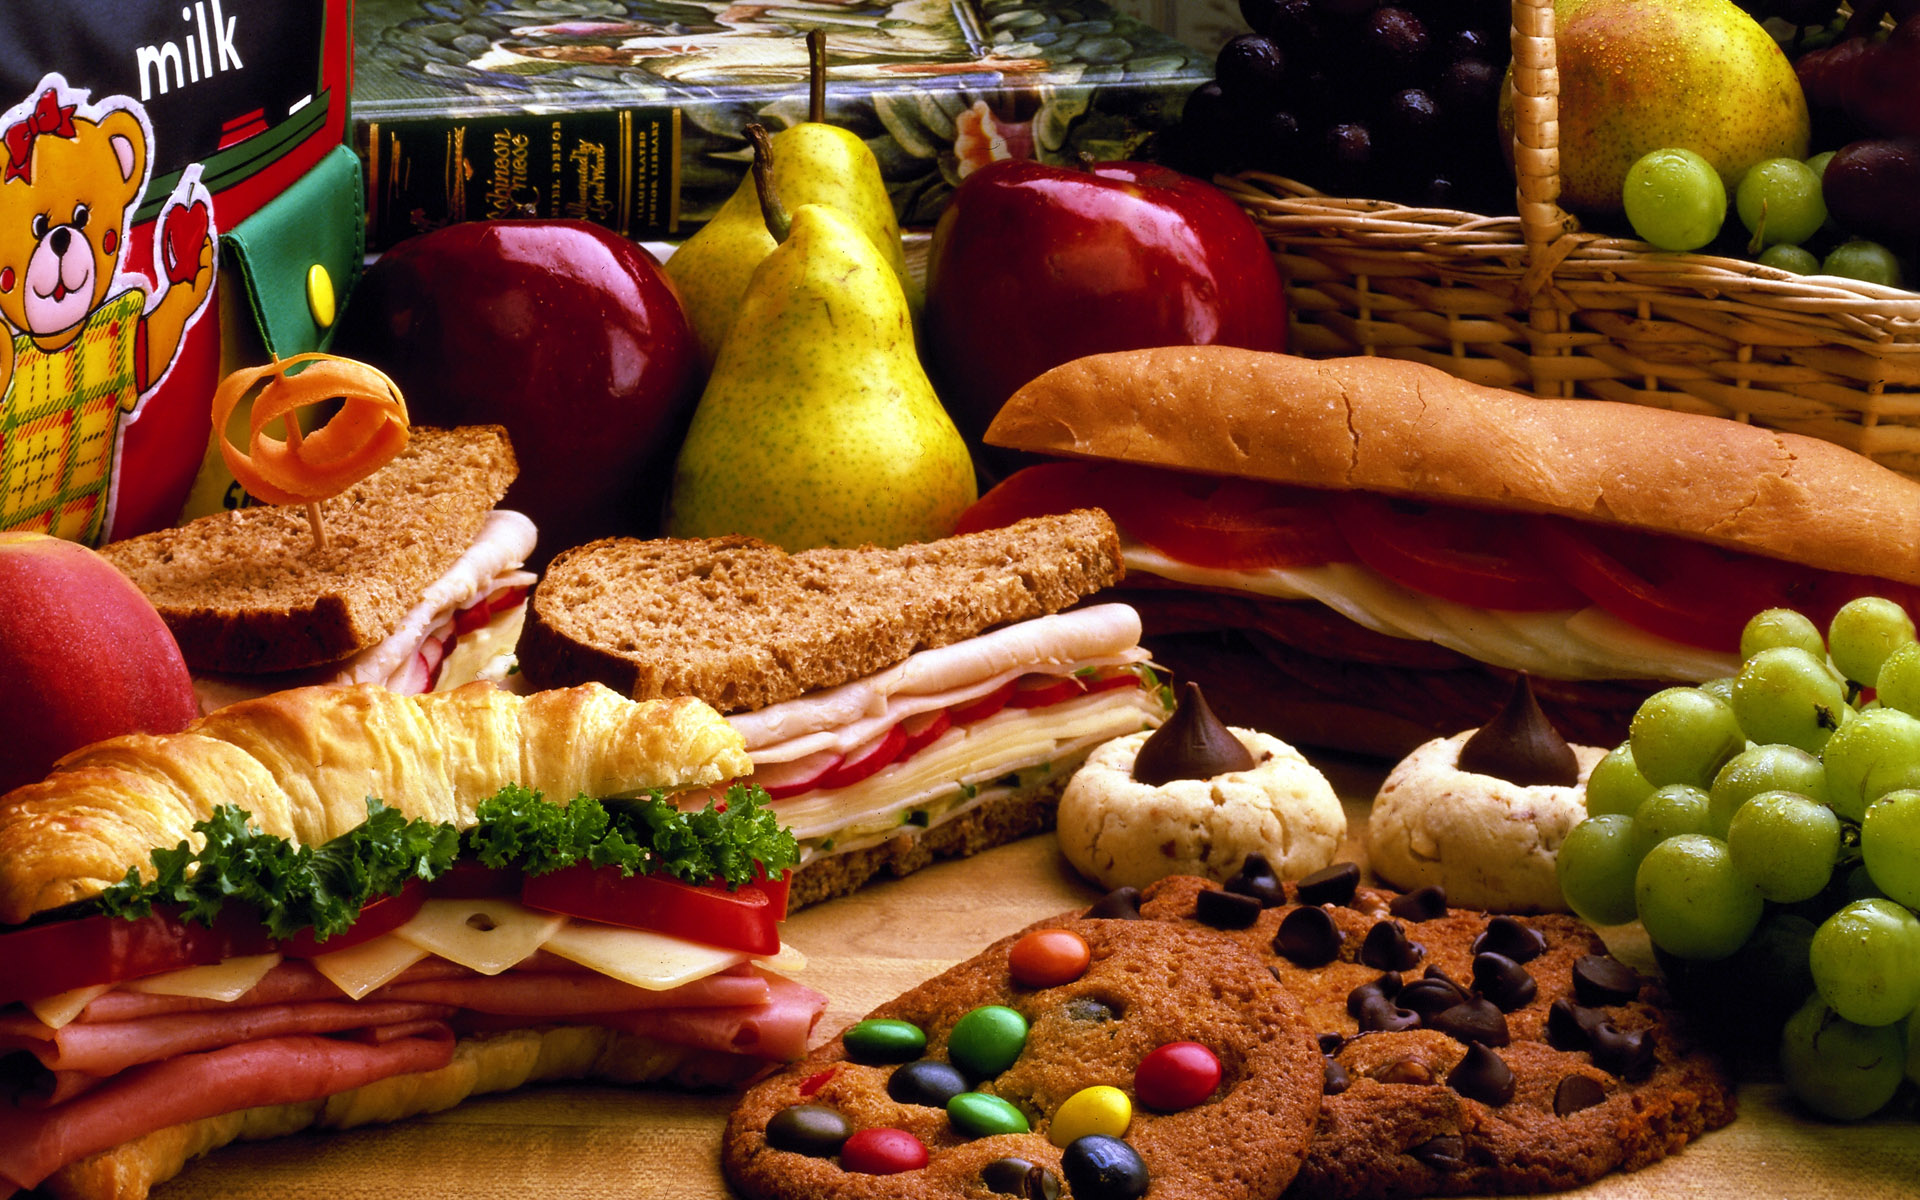
\includegraphics[width=\textwidth, height=0.35\textheight]{pictures/somefood.jpg}
\end{minipage}

\clearpage 

% Second recipe to test wheter the  variables are correctly handeled 
\begin{cleanrecipe}{Schrödingers Katze}
	\g{3}{Schödinger}
	\g{50}{Katze}
\end{cleanrecipe}

\iffalse
% Complete recipe example
\begin{recipe}
[% 
    preparationtime = {\unit[15]{min}},
    bakingtime={\unit[3-4]{h}},
    portion = {\portion{1}}
]
{Stired Onions}
    
    \graph
    {% pictures
    }
    
    \introduction{%
        Stired onions are actually really easy to make, even though they are often not done properly and many people are having trouble getting them right and not burning them. In this recipe, it will be almost impossible to burn them, they will be delicious, but on the downside it will take a really long time to make them.
    }
    
    \ingredients{%
        & Onions\\
        & Butter
    }
    
    \preparation{%
        \step Peel and cut the onions. The shape does not really matter, although you will mostly want little dice. For practise and some recipes, e.g. burgers, hoever you should use rings or half rings. The less thick the onios are cut, the less time this recipe will take. But make no mistake: As most of whats happening to the onions will take its time, no matter how thin the onions are sliced, it will always take quite long.
        
        \step Let the butter melt in a big pot. Seriously, you want a really big pot. A middle to big sized pan can also be used. Ideally the onions will just cover the bottom of the pot/pan. Most crucial in this will be the temperature. It should never be over 80\textcelcius, you will actually want it to be at around 60\textcelcius. The onions will at first not seem to change at all, and they shouldn't. But after about 3-4 hours, the onions will be perfect.
        
        \step Every now and then you will want to stir. This makes this recipe a bit tedious, as you are bound to the kitchen, and can only be away for so long. I would recommend stiring every 15 minutes. Depending on the type of pan or pot however this time will vary (a pan for example will lose more heat and thus will require more time to get the onions done but on the other hand you will get more time in between stirings).
        
        \step The onions are done when they are glassy and -depending on the type of onion- brownish-golden.
    }
    
    \hint{%
        Set alarms on your smartphone to not forget stirring.
    }
    
\end{recipe}
\fi